\ylDisplay{Peegel} % Ülesande nimi
{Tundmatu autor} % Autor
{lõppvoor} % Voor
{2012} % Aasta
{P 8} % Ülesande nr.
{1} % Raskustase
{
% Teema: Valgusõpetus
\ifStatement
Joonisel on näidatud optiline süsteem, mis koosneb peeglist, koondavast läätsest, esemest ja valgust blokeerivast barjäärist. Konstrueerige lisalehel eseme tõeline kujutis.
\begin{center}
	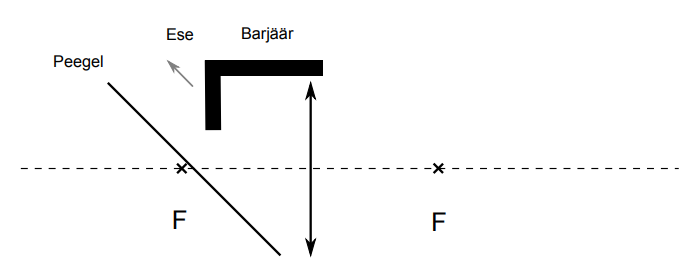
\includegraphics[width=0.5\linewidth]{2012-v3p-08-yl.PNG}
\end{center}
\fi
\ifHint
Kõige lihtsam viis ülesande lahendamiseks on kõigepealt konstrueerida eseme (näiv) kujutis peeglis ja konstrueerida sellest läätse abil tekkiv kujutis. Barjäär tagab, et tekib ainult üks tõeline kujutis.
\fi
\ifSolution
Kõige lihtsam viis ülesande lahendamiseks on kõigepealt konstrueerida eseme (näiv) kujutis peeglis ja konstrueerida sellest läätse abil tekkiv kujutis. Barjäär tagab, et tekib ainult üks tõeline kujutis.
\begin{center}
	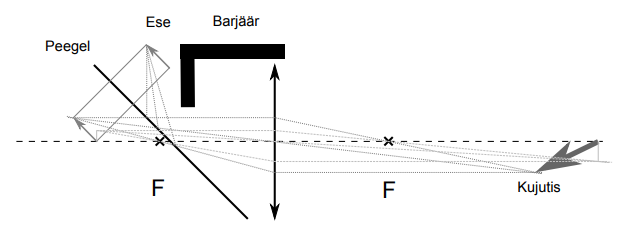
\includegraphics[width=0.5\linewidth]{2012-v3p-08-lah.PNG}
\end{center}
\fi
}
